../cictikz/src/cictikz/data/tex/cictikz_preamble.tex

% Carrier concentrations along the MOSFET: electrons (blue) high in the
% n+ source/drain, holes (red) high in the p bulk under the gate.

\definecolor{ncurve}{RGB}{40,40,140}
\definecolor{pcurve}{RGB}{220,60,50}
\definecolor{regg}{RGB}{70,130,60}
\definecolor{lblred}{RGB}{160,25,35}

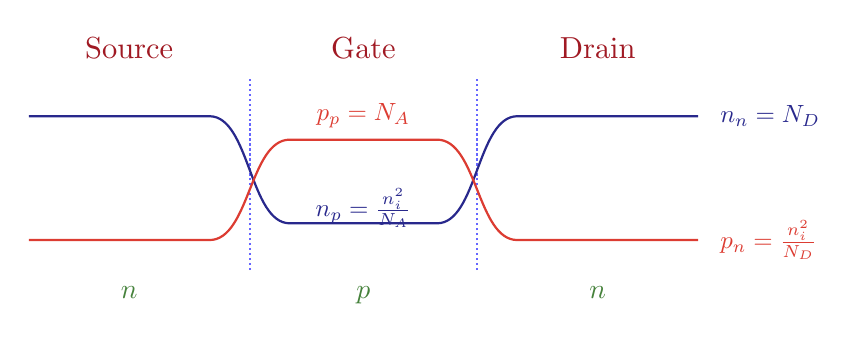
\begin{tikzpicture}[scale=0.85]

  % region dividers
  \draw[densely dotted, thick, blue!60] (3.3,0.2) -- (3.3,3.1);
  \draw[densely dotted, thick, blue!60] (6.7,0.2) -- (6.7,3.1);

  % electron concentration
  \draw[ncurve, thick]
    (0,2.5) -- (2.7,2.5) .. controls (3.3,2.5) and (3.3,0.9) .. (3.9,0.9)
    -- (6.1,0.9) .. controls (6.7,0.9) and (6.7,2.5) .. (7.3,2.5) -- (10,2.5);
  % hole concentration
  \draw[pcurve, thick]
    (0,0.65) -- (2.7,0.65) .. controls (3.3,0.65) and (3.3,2.15) .. (3.9,2.15)
    -- (6.1,2.15) .. controls (6.7,2.15) and (6.7,0.65) .. (7.3,0.65) -- (10,0.65);

  % concentration labels
  \node[pcurve, anchor=south, scale=0.9] at (5.0,2.2) {$p_p = N_A$};
  \node[ncurve, anchor=north, scale=0.9] at (5.0,1.55) {$n_p = \frac{n_i^2}{N_A}$};
  \node[ncurve, anchor=west, scale=0.9] at (10.2,2.5) {$n_n = N_D$};
  \node[pcurve, anchor=west, scale=0.9] at (10.2,0.65) {$p_n = \frac{n_i^2}{N_D}$};

  % region labels
  \node[lblred, anchor=south, scale=1.1] at (1.5,3.2) {Source};
  \node[lblred, anchor=south, scale=1.1] at (5.0,3.2) {Gate};
  \node[lblred, anchor=south, scale=1.1] at (8.5,3.2) {Drain};
  \node[regg, anchor=north, scale=1.0] at (1.5,0.1) {$n$};
  \node[regg, anchor=north, scale=1.0] at (5.0,0.1) {$p$};
  \node[regg, anchor=north, scale=1.0] at (8.5,0.1) {$n$};

\end{tikzpicture}
\end{document}
